\subsection{Samples}

\frame{\tableofcontents[currentsubsection]}

\begin{frame}
  \frametitle{WAV Files}
  \begin{itemize}
    \item In essence, a WAV file is a series of values which represent the amplitudes of a wave
  \end{itemize}
  \begin{center}
    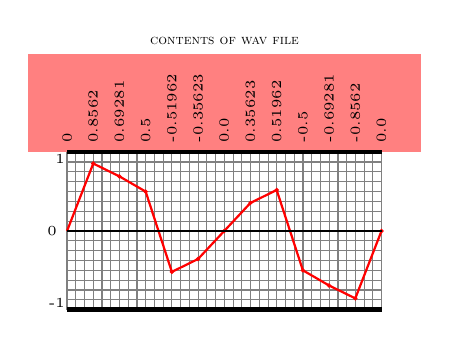
\begin{tikzpicture}
      \path[fill=red!50] (-0.5,1) rectangle (4.5,2.25);
      \node[anchor=south,font=\scshape\tiny] at (2,2.25) {contents of wav file};

      \draw[thin,gray] (0,-1) grid[xstep=0.111cm,ystep=0.125cm] (4,1);

      \foreach[evaluate={0.7*sin(2*\x)+0.2*sin(5*\x)+0.3*sin(13*\x)} as \y,
               remember=\y as \lasty (initially 0),
               remember=\x as \lastx (initially 0)] \x in {30,60,...,360} {
        \draw[fill,red] (\x*0.0111,\y) circle [radius=0.02cm];
        \node[right,font=\tiny,rotate=90] at (\x*0.0111,1) {\y};
        \draw[thick,red] (\lastx*0.0111,\lasty) -- (\x*0.0111,\y);
      }

      \node[right,font=\tiny,rotate=90] at (0,1) {0};

      \draw[ultra thick] (0,1) -- (4,1) node[at start,anchor=north east,inner sep=0pt,font=\tiny] {1};
      \draw[thick] (0,0) -- (4,0) node[at start,anchor=east,font=\tiny] {0};
      \draw[ultra thick] (0,-1) -- (4,-1) node[at start,anchor=south east,inner sep=0pt,font=\tiny] {-1};
    \end{tikzpicture}
  \end{center}
\end{frame}

\begin{frame}
  \frametitle{WAV Files}
  \begin{itemize}
  \item However, WAV files do not use floating points numbers
    \item WAV files use integers
    \item They range from 0 to 255 for 8 bit WAVs
    \item Or \num{-32768} to \num{+32768} for 16 bit WAVs
  \end{itemize}
  \begin{overprint}
    \onslide<1>
    \begin{center}
      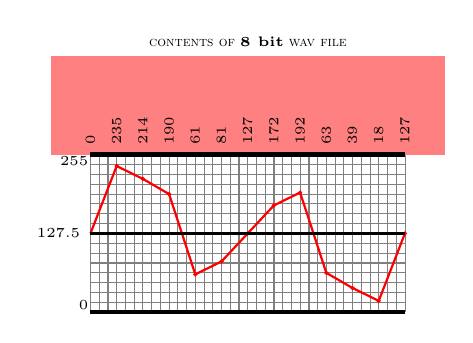
\begin{tikzpicture}
        \path[fill=red!50] (-0.5,1) rectangle (4.5,2.25);
        \node[anchor=south,font=\scshape\tiny] at (2,2.25) {contents of \textbf{8 bit} wav file};

        \draw[thin,gray] (0,-1) grid[xstep=0.111cm,ystep=0.125cm] (4,1);

        \foreach[evaluate={0.7*sin(2*\x)+0.2*sin(5*\x)+0.3*sin(13*\x)} as \y,
                 remember=\y as \lasty (initially 0),
                 remember=\x as \lastx (initially 0),
                 evaluate={int(\y*127+127)} as \v] \x in {30,60,...,360} {
          \draw[fill,red] (\x*0.0111,\y) circle [radius=0.02cm];
          \node[right,font=\tiny,rotate=90] at (\x*0.0111,1) {\v};
          \draw[thick,red] (\lastx*0.0111,\lasty) -- (\x*0.0111,\y);
        }

        \node[right,font=\tiny,rotate=90] at (0,1) {0};

        \draw[ultra thick] (0,1) -- (4,1) node[at start,anchor=north east,inner sep=0pt,font=\tiny] {255};
        \draw[thick] (0,0) -- (4,0) node[at start,anchor=east,font=\tiny] {127.5};
        \draw[ultra thick] (0,-1) -- (4,-1) node[at start,anchor=south east,inner sep=0pt,font=\tiny] {0};
      \end{tikzpicture}
    \end{center}
    \onslide<2>
    \begin{center}
      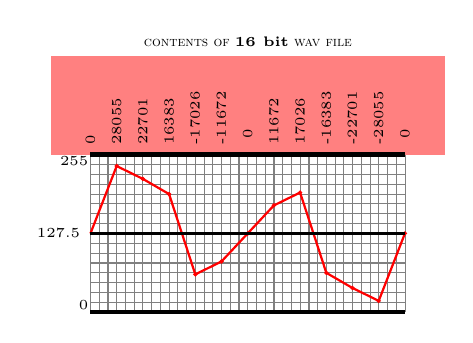
\begin{tikzpicture}
        \path[fill=red!50] (-0.5,1) rectangle (4.5,2.25);
        \node[anchor=south,font=\scshape\tiny] at (2,2.25) {contents of \textbf{16 bit} wav file};

        \draw[thin,gray] (0,-1) grid[xstep=0.111cm,ystep=0.125cm] (4,1);

        \foreach[evaluate={0.7*sin(2*\x)+0.2*sin(5*\x)+0.3*sin(13*\x)} as \y,
                 remember=\y as \lasty (initially 0),
                 remember=\x as \lastx (initially 0),
                 evaluate={\y*32.767} as \v,
                 evaluate={int(\v)} as \thousands,
                 evaluate={int(abs(\v-\thousands)*1000)} as \rest] \x in {30,60,...,360} {
          \draw[fill,red] (\x*0.0111,\y) circle [radius=0.02cm];
          \node[right,font=\tiny,rotate=90] at (\x*0.0111,1) {\ifnum\thousands=0
                                                                {}
                                                              \else\thousands\fi
                                                              \ifnum\rest=0
                                                                0
                                                              \else
                                                              \ifnum\rest<10 00\rest
                                                              \else\ifnum\rest<100 0\rest
                                                                         \else\rest\fi\fi\fi};
          \draw[thick,red] (\lastx*0.0111,\lasty) -- (\x*0.0111,\y);
        }

        \node[right,font=\tiny,rotate=90] at (0,1) {0};

        \draw[ultra thick] (0,1) -- (4,1) node[at start,anchor=north east,inner sep=0pt,font=\tiny] {255};
        \draw[thick] (0,0) -- (4,0) node[at start,anchor=east,font=\tiny] {127.5};
        \draw[ultra thick] (0,-1) -- (4,-1) node[at start,anchor=south east,inner sep=0pt,font=\tiny] {0};
      \end{tikzpicture}
    \end{center}
  \end{overprint}
\end{frame}

\begin{frame}
  \frametitle{Overview Update}
  \begin{center}
    \begin{tikzpicture}[milestone/.style={drop shadow,draw,fill=red!50,minimum height=7.5mm,minimum width=1cm,font=\tiny\scshape},
                        link/.style={-latex,thick},
                        arrow/.style={blue,ultra thick,-{Stealth[]}},
                        scale=.8,transform shape]
      \node[milestone] (uint8) at (0,0) {\texttt{Stream<uint8>}};
      \node[milestone] (int16) at ($ (uint8) + (2,1) $) {\texttt{Stream<int16>}};
      \node[milestone] (double) at ($ (uint8) + (4,0) $) {\texttt{Stream<double>}};
      \node[milestone] (wave) at ($ (double) + (3,0) $) {\texttt{Wave}};

      \draw[link] (uint8) |- (int16);
      \draw[link] (int16) -| (double);
      \draw[link] (uint8) -- (double);
      \draw[link] (double) -- (wave);

      \visible<1>{
        \coordinate (link middle) at ($ (uint8.east) ! 0.5 ! (double.west) $);
        \draw[arrow] ($ (link middle) - (0,1.5) $) -- (link middle);
      }
      \visible<2>{
        \draw[arrow] ($ (int16) + (0,1.5) $) -- (int16);
      }
    \end{tikzpicture}
  \end{center}
  \begin{overprint}
    \onslide<1>
    \begin{itemize}
      \item If the WAV file contains 8 bit samples, we can directly convert them to \texttt{double}s
      \item Convert $[0,255]$ to $[-1,1]$
            \begin{center}
              \texttt{byte / 127.5 - 1}
            \end{center}
    \end{itemize}

    \onslide<2>
    \begin{itemize}
      \item If the WAV file contains 16 bit samples, however, we must first group pairs of bytes together to
            form the 16 bit values
            \begin{center} \ttfamily
              sample = byte1 | (byte2 << 8) 
            \end{center}
      \item Convert $[-32768,32767]$ to $[-1,1]$
            \begin{center} \ttfamily
              (1 + 2 * sample) / 65535.0
            \end{center}
    \end{itemize}
  \end{overprint}
\end{frame}



%%% Local Variables:
%%% mode: latex
%%% TeX-master: "sound"
%%% End:
